\documentclass[AMA,STIX1COL]{WileyNJD-v2}

\usepackage{mathtools}
\usepackage{tuda-pgfplots}
\usepackage{siunitx}
\usepackage[european]{circuitikz}
\usepackage{subcaption}

\articletype{Original Article}

\received{}
\revised{}
\accepted{}

\raggedbottom
\newcommand{\mb}[1]{\mathbf{#1}}
\newcommand{\mbt}[1]{\tilde{\mathbf{#1}}}
\newcommand{\mbb}[1]{\bar{\mathbf{#1}}}
\newcommand{\mbh}[1]{\hat{\mathbf{#1}}}
\newcommand{\mr}[1]{\mathrm{#1}}
\newcommand{\T}{{\!\top}}
\newcommand{\ddt}{\frac{\mathrm{d}}{\mathrm{d}t}}
\newcommand{\A}[1]{\mb{A}_\mr{#1}}
\newcommand{\AT}[1]{\mb{A}_\mr{#1}^{\T}}
\newcommand{\qC}{\mb{q}_\mr{C}}
\newcommand{\gR}{\mb{g}_\mr{R}}
\newcommand{\phiL}{\boldsymbol{\phi}_\mr{L}}
\newcommand{\vphi}{\boldsymbol{\varphi}}
\renewcommand{\i}[1]{\mb{i}_\mr{#1}}
\renewcommand{\v}[1]{\mb{v}_\mr{#1}}

\usetikzlibrary{external}
\tikzexternalize

\begin{document}

\title{Index-aware learning of circuits}

\author[1]{Idoia Cortes Garcia}
\author[1,2]{Peter Förster*}
\author[2]{Lennart Jansen}
\author[1]{Wil Schilders}
\author[2]{Sebastian Schöps}
% \authormark{}
\address[1]{\orgname{Eindhoven University of Technology}, \orgaddress{\country{Netherlands}}}
\address[2]{\orgname{Technical University of Darmstadt}, \orgaddress{\country{Germany}}}
\corres{*Peter Förster, Eindhoven University of Technology. \email{p.f.forster@tue.nl}}
% \presentaddress{}

\abstract[Summary]{Electrical circuits are present in a variety of technologies, making their design an important part of computer aided engineering. The growing number of tunable parameters that affect the final design leads to a need for new approaches of quantifying their impact. Machine learning may play a key role in this regard, however current approaches often make suboptimal use of existing knowledge about the system at hand. In terms of circuits, their description via modified nodal analysis is well-understood. This particular formulation leads to systems of differential-algebraic equations (DAEs) which bring with them a number of peculiarities, e.g. hidden constraints that the solution needs to fulfill. We aim to use the recently introduced dissection concept for DAEs that can decouple a given system into ordinary differential equations, only depending on differential variables, and purely algebraic equations that describe the relations between differential and algebraic variables. The idea then is to only learn the differential variables and reconstruct the algebraic ones using the relations from the decoupling. This approach guarantees that the algebraic constraints are fulfilled up to the accuracy of the nonlinear system solver, which represents the main benefit highlighted in this article.}

\keywords{electrical circuits, differential-algebraic equations, modified nodal analysis, dissection concept, machine learning}

\maketitle

\section{Introduction}
\label{sec:int}
Design optimization and uncertainty quantification are ubiquitous tools of modern computer aided  engineering. Due to the ever-increasing complexity of engineering systems, machine learning techniques have gained popularity for constructing surrogate models when the objective function becomes expensive to evaluate and a large number of (design or uncertainty) parameters are present. In these cases, classical model order reduction techniques\cite{schilders2008} or function approximation approaches\cite{xiu2010} suffer from the curse of dimensionality: the number of operations to construct and the memory required to store the model grow exponentially with respect to the number of parameters. Experimental and in some cases even theoretical evidence\cite{beneventano2020} shows that machine learning approaches may be able to overcome the curse of dimensionality and provide surrogates that are fast to evaluate, while requiring comparably little data.

In the particular case of electrical circuit design, neural networks have been used for design optimization for over 20 years\cite{zaabab1995,fang2000}. More recently, Gaussian process regression has been employed for both uncertainty quantification and design optimization during analog integrated circuit design\cite{wang2018,sanabria2020}. The commonality between these approaches is that they focus on the learning part: they aim to provide a computationally efficient and accurate surrogate, given data produced by some circuit simulation software. Thus, they all treat the circuit simulator as a black box that simply provides the data which is then used for constructing the surrogate. In contrast, we want to exploit the known structure that underlies the equations describing electrical circuits.

More specifically, we consider the modified nodal analysis\cite{ho1975} (MNA). MNA is one of the most popular circuit descriptions and lies at the center of SPICE-like simulation software such as LTspice\cite{ltspice}, Xyce\cite{xyce} and PSpice\cite{pspice}. Applying MNA to a given circuit leads to systems of differential-algebraic equations (DAEs), which can generally be written as systems of implicit differential equations \cite{denk1991}
\begin{align*}
    \mb{f}(\mb{x}', \mb{x}, t, \mb{p}) = \mb{0}, \quad \mb{x}(0) = \mb{x}_0,
\end{align*}
where the Jacobian $\mb{J}_{\mb{x}'}(\mb{f})$, of $\mb{f}$ w.r.t.~$\mb{x}'$, is singular and $\mb{p}$ are the design or uncertainty parameters. To give a more intuitive description, one can think of DAEs as ordinary differential equations (ODEs) that are constrained to a manifold determined by (hidden) constraints on the solution variables. Multiple so-called index concepts were introduced in order to characterize the difficulties that appear in the context of DAEs. A reference by Mehrmann\cite{mehrmann2015} outlines some of the most prominent, including the differentiation, tractability, strangeness and perturbation indices. For all of these, the index $\nu \in \mathbb{N}$ depends on structural properties of the DAE and (informally) measures the degree of difficulty associated with solving it. In this sense, higher index DAEs usually lead to more problems, both analytically and numerically.

Various relationships between the indices, including situations when they coincide, are also known\cite{mehrmann2015} and the structure and index of MNA are well understood for both independent sources\cite{tischendorf1999} and controlled sources\cite{estevez2000ijcta}. Rather recently, the dissection concept was introduced\cite{jansen2014}. It combines features of the strangeness and tractability indices to decouple a DAE into an ODE and a set of purely algebraic equations. In particular, the entire dynamics of the solution may then be found only using the ODE. We aim to use this dissection concept to propose an approach for learning electrical circuits more accurately and efficiently.

In the following, \autoref{sec:mna} introduces MNA in more detail and states some well-known related results. Afterwards, \autoref{sec:dc} outlines the dissection concept and showcases its properties using small example circuits. The same examples are then used to present the new approach on an abstract level in \autoref{sec:ial} and on a numerical level in \autoref{sec:ne}, where we also showcase an alternative method that trades some of the accuracy of our approach for an easier implementation. Preliminary conclusions about the effectiveness of our approach and future research directions are given in \autoref{sec:cfr}.

\section{Modified nodal analysis}
\label{sec:mna}
We begin by looking at the system of DAEs that results from MNA. From here onward we will disregard controlled sources. As these are of crucial importance for engineering applications however, we will state whether extensions including controlled sources are available or missing at the appropriate times. Borrowing the notation from Tischendorf\cite{tischendorf1999}, and only explicitly expressing the time dependence of independent sources for brevity, the system of MNA reads
\begin{subequations}
    \label{eq:mnai}
    \begin{align}
            \A{C} \ddt \qC \big( \AT{C} \vphi \big) + \A{R} \gR \big( \AT{R} \vphi \big) + \A{L} \i{L} + \A{V} \i{V} + \A{I} \i{s}(t) &= \mb{0}\\ 
            \ddt \phiL \big( \i{L} \big) - \AT{L} \vphi &= \mb{0}\\
            \AT{V} \vphi - \v{s}(t)&= \mb{0},
    \end{align}
\end{subequations}
where $\gR$, $\qC$ and $\phiL$ represent functions modeling resistive, capacitive or inductive devices respectively. The terms for independent current and voltage sources are given by $\i{s}(t)$ and $\v{s}(t)$, while $\vphi$ denotes the vector of nodal potentials and $\i{L} $, $\i{V}$ are the currents flowing through branches containing inductors or voltage sources respectively. The last ingredient is given by the incidence matrices $\A{*}$, where $*$ indicates the device type. These collect the branch to node relations of the underlying electrical network when considering the branches and nodes as edges and vertices of a graph. In the context of design optimization or uncertainty quantification, the device functions $\gR$, $\qC$ or $\phiL$ could e.g.~depend on (subsets of) the parameters $\mb{p}$.

In order to obtain a version of \eqref{eq:mnai} that is better suited to analysis and implementation, we consider the device function Jacobians
\begin{align}
    \mb{L}(\i{L}) \coloneqq \mb{J}_{\i{L}}(\phiL), \quad \mb{C} \big( \AT{C} \vphi \big) \coloneqq \mb{J}_{\AT{C} \vphi}(\qC) \label{eq:dfj},
\end{align}
where we use the same notation for the Jacobians as in \autoref{sec:int}. We also assume that the device function for resistors may be expressed as
\begin{align}
    \gR \big( \AT{R} \vphi \big) = \mb{G} \big( \AT{R} \vphi \big) \AT{R} \vphi \label{eq:dfr}.
\end{align}
In practice, this is accomplished by either considering the chordal (static) conductance $\frac{[\gR]_i}{[\AT{R} \vphi]_i}$ for each resistor $\mr{R}_i$ separately or by using the Jacobian $\mathbf{J}_{ \AT{R} \vphi}(\gR)$. Inserting \eqref{eq:dfj} and \eqref{eq:dfr} into the original system and writing it in matrix form yields
\begin{align}
    \begin{bmatrix}
        \A{C}^{\phantom{\T}} \mb{C} \big( \AT{C} \vphi \big) \AT{C} & &\\
        & \mb{L}(\i{L}) &\\
        & & \mb{0}
    \end{bmatrix} \ddt \begin{bmatrix}
        \vphi\\
        \i{L}\\
        \i{V}
    \end{bmatrix} + \begin{bmatrix}
        \A{R}^{\phantom{\T}} \mb{G} \big( \AT{R} \vphi \big) \AT{R} & \A{L} & \A{V}\\
        -\AT{L} & &\\
        -\AT{V} & &
    \end{bmatrix} \begin{bmatrix}
        \vphi\\
        \i{L}\\
        \i{V}
    \end{bmatrix} + \begin{bmatrix}
        \A{I} \i{s}(t)\\
        \mb{0}\\
        \v{s}(t)
    \end{bmatrix} = \mb{0} \label{eq:mnaii},
\end{align}
where we assume that $\qC$ and $\phiL$ do not explicitly depend on time. MNA is usually presented in the form of \eqref{eq:mnaii} and for it, there exists the following well-known topological index result.
\begin{quote}
    Assuming the matrix-valued functions $\mathbf{G}$, $\mathbf{L}$, $\mathbf{C}$ from \eqref{eq:dfj} and \eqref{eq:dfr} positive definite:
    \begin{enumerate}
        \item The index of \eqref{eq:mnaii} is $\nu \leq 2$.
        \item The index of \eqref{eq:mnaii} is $\nu \leq 1$, if and only if there are no loops consisting only of capacitors and voltage sources containing at least one voltage source and no cutsets consisting only of inductors and current sources.
    \end{enumerate}
    The result can be found in terms of the tractability index\cite{tischendorf1999}, the differentiation index \cite{estevez2000ijcta} and the dissection concept\cite{jansen2014}. % \cite[Theorem 4.28]{jansen2014}
\end{quote}
We remark that there also exist extensive results about when the index of MNA including controlled sources does not exceed $\nu = 2$\cite{estevez2000ijcta}.

\section{Dissection concept}
\label{sec:dc}
This section serves as a general introduction to the dissection concept and more specifically its application to MNA as given in \eqref{eq:mnaii}. Consider a linear DAE in standard form\cite{jansen2014},
\begin{align}
    \mb{M} \ddt \mb{x} + \mb{K} \mb{x} + \mb{f}(t) = \mb{0}, \quad \ker \mb{M} \supsetneq \{ \mb{0} \} \label{eq:dae},
\end{align}
where we again keep the time dependence of $\mb{x}$ implicit. We now demonstrate the first two steps of the dissection concept when applied to systems of the form of \eqref{eq:dae} and remark that although \eqref{eq:mnaii} is a nonlinear DAE, the decoupling still takes the same form in this case due to the special structure of MNA\cite{jansen2014}.

\subsection{Index one case}
Assuming $\mb{M} \in \mathbb{R}^{n \times m}$, we define four basis functions $\mb{P}$, $\mb{Q}$, $\mb{V}$, $\mb{W}$ such that
\begin{align*}
    \mr{im\, } \mb{Q} = \ker \mb{M}, \quad \mr{im\, } \mb{W} = \ker \mb{M}^{\T}
\end{align*}
and the columns of $\mb{P}$ and $\mb{Q}$ together form a basis of $\mathbb{R}^n$, while the columns of $\mb{V}$ and $\mb{W}$ together form a basis of $\mathbb{R}^m$.

\paragraph{Splitting the solution}
The key idea is to use the basis functions to split the solution $\mb{x}$ into two parts
\begin{align}
    \mb{x} = \mb{P} \mbt{x} + \mb{Q} \mbb{x} \label{eq:vs},
\end{align}
where $\tilde{\cdot}$ is used to indicate differential (dynamic) variables and $\bar{\cdot}$ signifies algebraic (fixed) variables. When inserting the splitting \eqref{eq:vs} into the general system \eqref{eq:dae} we observe the following
\begin{align}
    \mb{M} \mb{P} \ddt \mbt{x} + \mb{K} \mb{P} \mbt{x} + \mb{K} \mb{Q} \mbb{x} + \mb{f}(t) = \mb{0} \label{eq:rs}
\end{align}
and this motivates the notation, as only $\mbt{x}$ appears differentiated in time.

\paragraph{Splitting the system}
The procedure then continues by multiplying \eqref{eq:rs} with $\mb{V}^{\T}$ and $\mb{W}^{\T}$ from the left. This yields
\begin{subequations}
    \label{eq:io}
    \begin{align}
            \underbrace{\mb{V}^{\T} \mb{M} \mb{P}}_{\eqqcolon \mbt{M}} \ddt \mbt{x} + \underbrace{\mb{V}^{\T} \mb{K} \mb{P}}_{\eqqcolon \mbt{K}_\mb{P}} \mbt{x} + \underbrace{\mb{V}^{\T} \mb{K} \mb{Q}}_{\eqqcolon \mbt{K}_\mb{Q}} \mbb{x} + \underbrace{\mb{V}^{\T} \mb{f}(t)}_{\eqqcolon \mbt{f}(t)} &= \mb{0} \label{eq:ioa}\\
            \underbrace{\mb{W}^{\T} \mb{K} \mb{P}}_{\eqqcolon \mbb{K}_\mb{P}} \mbt{x} + \underbrace{\mb{W}^{\T} \mb{K} \mb{Q}}_{\eqqcolon \mbb{K}_\mb{Q}} \mbb{x} + \underbrace{\mb{W}^{\T} \mb{f}(t)}_{\eqqcolon \mbb{f}(t)} &= \mb{0} \label{eq:iob},
    \end{align}
\end{subequations}
where we also introduce shorthands for the arising products. The key observations regarding \eqref{eq:io} are the following: $\mbt{M}$ is regular by construction, thus if $\mbb{K}_\mb{Q}$ is regular, \eqref{eq:iob} gives a purely algebraic equation for $\mbb{x}$ in terms of $\mbt{x}$. Solving this equation for $\mbb{x}$ and inserting the solution into \eqref{eq:ioa} then yields an ODE in the differential variables $\mbt{x}$. In this case, the \textbf{(dissection) index} of the DAE is defined to be $\nu = 1$.

\subsection{Index two case}
There are of course many DAEs, including those described by MNA, which have a higher index. For these the dissection concept proceeds by introducing additional basis functions and continuing the splitting process in a similar fashion.

\paragraph{Splitting the algebraic variables}
We begin by considering basis functions $\mbb{P}, \mbb{Q}, \mbb{V}, \mbb{W}$ of $\mbb{K}_\mb{Q}$ and split the algebraic variables $\mbb{x}$ further as follows
\begin{align}
    \mbb{x} = \mbb{P} \mbb{x}_\mb{P} + \mbb{Q} \mbb{x}_\mb{Q} \label{eq:xb}.
\end{align}
Inserting this decomposition into \eqref{eq:iob} and multiplying once by $\mbb{V}^{\T}$ and $\mbb{W}^{\T}$ from the left yields
\begin{subequations}
    \label{eq:iti}
    \begin{align}
        \mbb{V}^{\T} \mbb{K}_\mb{P} \mbt{x} + \mbb{V}^{\T} \mbb{K}_\mb{Q} \mbb{P} \mbb{x}_\mb{P} + \mbb{V}^{\T} \mbb{f}(t) &= \mb{0} \label{eq:itia}\\
        \mbb{W}^{\T} \mbb{K}_\mb{P} \mbt{x} + \mbb{W}^{\T} \mbb{f}(t) &= \mb{0} \label{eq:itib}.
    \end{align}
\end{subequations}

\paragraph{Splitting the differential variables}
We now need basis functions $\mbt{P}, \mbt{Q}$ of $\mbb{W}^{\T} \mbb{K}_\mb{P}$ to split the differential variables $\mbt{x}$ as
\begin{align}
    \mbt{x} = \mbt{P} \mbt{x}_\mb{P} +
    \mbt{Q} \mbt{x}_\mb{Q} \label{eq:xt}
\end{align}
and inserting this splitting into \eqref{eq:itib} then allows for an explicit description of $\mbt{x}_\mb{P}$
\begin{align*}
    \mbt{x}_\mb{P} = -\big( \mbb{W}^{\T} \mbb{K}_\mb{P} \mbt{P} \big)^{-1} \mbb{W}^{\T} \mbb{f}(t) \eqqcolon \mbt{f}_\mb{P}(t),
\end{align*}
since $\mbb{W}^{\T} \mbb{K}_\mb{P} \mbt{P}$ is assumed to be regular (otherwise the DAE is underdetermined\cite{jansen2014}).

\paragraph{Splitting the solution}
Similarly, inserting \eqref{eq:xt} into \eqref{eq:itia} gives a description of $\mbb{x}_\mb{P}$ in terms of $\mbt{x}_\mb{Q}$ as $\mbb{V}^{\T} \mbb{K}_\mb{Q} \mbb{P}$ is guaranteed to be nonsingular
\begin{align*}
    \mbb{x}_\mb{P} = -\big( \mbb{V}^{\T} \mbb{K}_\mb{Q} \mbb{P} \big)^{-1} \big( \mbb{V}^{\T} \mbb{K}_\mb{P} \mbt{Q} \mbt{x}_\mb{Q} + \mbb{V}^{\T} \mbb{K}_\mb{P} \mbt{P} \mbt{x}_\mb{P} + \mbb{V}^{\T} \mbb{f}(t) \big) \eqqcolon \mbb{K} \mbt{x}_\mb{Q} + \mbb{f}_\mb{P}(t).
\end{align*}
Expanding $\mbt{x}$ and $\mbb{x}$ in \eqref{eq:ioa}, according to \eqref{eq:xb} and \eqref{eq:xt} respectively, and using the above expressions for $\mbt{x}_\mb{P}$ and $\mbb{x}_\mb{P}$ gives
\begin{align}
    \mbt{M} \mbt{Q} \ddt \mbt{x}_\mb{Q} + \big( \mbt{K}_\mb{P} \mbt{Q} + \mbt{K}_\mb{Q} \mbb{P} \mbb{K} \big) \mbt{x}_\mb{Q} + \mbt{K}_\mb{Q} \mbb{Q} \mbb{x}_\mb{Q} + \mbh{f}(t) = \mb{0} \label{eq:itii},
\end{align}
where we define
\begin{align*}
    \mbh{f}(t) \coloneqq \mbt{M} \mbt{P} \ddt \mbt{f}_\mb{P}(t) + \mbt{K}_\mb{P} \mbt{P} \mbt{f}_\mb{P}(t) + \mbt{K}_\mb{Q} \mbb{P} \mbb{f}_\mb{P}(t) + \mbt{f}(t).
\end{align*}

\paragraph{Splitting the system}
Finally, we require basis functions $\mbt{V}$ and $\mbt{W}$ of $\mbt{M} \mbt{Q}$. Multiplying \eqref{eq:itii} from the left by $\mbt{V}^{\T}$ and $\mbt{W}^{\T}$ and redefining $\mbt{x}_2 \coloneqq \mbt{x}_\mb{Q}$ and $\mbb{x}_2 \coloneqq \mbb{x}_\mb{Q}$ yields
\begin{subequations}
    \label{eq:itiii}
    \begin{align}
            \underbrace{\mbt{V}^{\T} \mbt{M} \mbt{Q}}_{\eqqcolon \mbt{M}_2} \ddt \mbt{x}_2 + \underbrace{\mbt{V}^{\T} \big( \mbt{K}_\mb{P} \mbt{Q} + \mbt{K}_\mb{Q} \mbb{P} \mbb{K} \big)}_{\eqqcolon \mbt{K}_{\mb{P}_2}} \mbt{x}_2 + \underbrace{\mbt{V}^{\T} \mbt{K}_\mb{Q} \mbb{Q}}_{\eqqcolon \mbt{K}_{\mb{Q}_2}} \mbb{x}_2 + \underbrace{\mbt{V}^{\T} \mbh{f}(t)}_{\eqqcolon \mbt{f}_2(t)} &= \mb{0} \label{eq:itiiia}\\
            \underbrace{\mbt{W}^{\T} \big( \mbt{K}_\mb{P} \mbt{Q} + \mbt{K}_\mb{Q} \mbb{P} \mbb{K} \big)}_{\eqqcolon \mbb{K}_{\mb{P}_2}} \mbt{x}_2 + \underbrace{\mbt{W}^{\T} \mbt{K}_\mb{Q} \mbb{Q}}_{\eqqcolon \mbb{K}_{\mb{Q}_2}} \mbb{x}_2 + \underbrace{\mbt{W}^{\T} \mbh{f}(t)}_{\eqqcolon \mbb{f}_2(t)} &= \mb{0}. \label{eq:itiiib}
    \end{align}
\end{subequations}
We observe that \eqref{eq:itiii} is of the same form as \eqref{eq:io} and that $\mbt{M}_2$ is again regular by construction. Therefore, if $\mbb{K}_{\mb{Q}_2}$ is also regular we can extract an ODE analogous to the previous case by solving \eqref{eq:itiiib} for $\mbb{x}_2$ (in terms of $\mbt{x}_2$) and inserting that solution into \eqref{eq:itiiia}. The DAE is then said to have \textbf{dissection index} $\nu = 2$ and we call $\mbt{x}_2$ the differential variables and $\mbb{x}_2$ the algebraic variables. Furthermore, since \eqref{eq:itiii} and \eqref{eq:io} are structurally identical, we may simply apply the second step of the decoupling procedure to \eqref{eq:itiii} in order to deal with even higher index DAEs.

To clarify the naming convention for the following sections, we call $\mbt{x}_2$ and $\mbb{x}_2$ the purely differential and algebraic variables of an index two DAE respectively, whereas $\mbb{x}$ denotes the explicit (obvious) algebraic variables and $\mbt{x}$ still contains hidden (implicit) algebraic variables that are identified in the second step of the dissection concept.

\subsection{Dissection concept and MNA}
\label{subsec:dcmna}
Before we consider example circuits, we take a brief look at the first step of the dissection concept for MNA. For this, we recall the system of MNA \eqref{eq:mnaii}
\begin{align*}
    \begin{bmatrix}
        \A{C}^{\phantom{\T}} \mb{C} \big( \AT{C} \vphi \big) \AT{C} & &\\
        & \mb{L}(\i{L}) &\\
        & & \mb{0}
    \end{bmatrix} \ddt \begin{bmatrix}
        \vphi\\
        \i{L}\\
        \i{V}
    \end{bmatrix} + \begin{bmatrix}
        \A{R}^{\phantom{\T}} \mb{G} \big( \AT{R} \vphi \big) \AT{R} & \A{L} & \A{V}\\
        -\AT{L} & &\\
        -\AT{V} & &
    \end{bmatrix} \begin{bmatrix}
        \vphi\\
        \i{L}\\
        \i{V}
    \end{bmatrix} + \begin{bmatrix}
        \A{I} \i{s}(t)\\
        \mb{0}\\
        \v{s}(t)
    \end{bmatrix} = \mb{0}
\end{align*}
and determine the basis functions $\mb{P}$ and $\mb{Q}$. Taking into account the standard assumption, compare \autoref{sec:mna}, that $\mb{L}(\i{L})$ and $\mb{C} \big( \AT{C} \vphi \big)$ are positive definite, we find\cite{jansen2014}
\begin{align*}
    \mb{Q} = \begin{bmatrix}
        \mb{Q}_\mr{C} &\\
        & \mb{0}\\
        & \mb{I}
    \end{bmatrix}, \quad \mb{P} = \begin{bmatrix}
        \mb{P}_\mr{C} &\\
        & \mb{I}\\
        & \mb{0}
    \end{bmatrix},
\end{align*}
where $\mr{im\, } \mb{Q}_\mr{C} = \ker \AT{C}$, $\mb{0}$ and $\mb{I}$ are zero and identity matrices of appropriate dimension and the columns of $\mb{Q}_\mr{C}$ and $\mb{P}_\mr{C}$ together form a basis of $\mathbb{R}^{n_\varphi}$ with $n_\varphi$ the dimension of $\vphi$. The description of $\mb{Q}_\mr{C}$ results from the fact that (with $\mb{y} \coloneqq \AT{C} \mb{x}$)
\begin{align*}
    \mb{x}^{\T} \A{C}^{\phantom{\T}} \mb{C} \big( \AT{C} \vphi \big) \AT{C} \mb{x} = \mb{y}^{\T} \mb{C} \big( \AT{C} \vphi \big) \mb{y} > 0, \quad \forall \mb{y} \in \mathbb{R}^{n_\varphi} \setminus \{ \mb{0} \},
\end{align*}
since $\mb{C} \big( \AT{C} \vphi \big)$ is positive definite and hence the kernel of $\A{C}^{\phantom{\T}} \mb{C} \big( \AT{C} \vphi \big) \AT{C}$ is determined by the kernel of $\AT{C}$. As $\A{C}$ is an incidence (constant) matrix, we find that $\mb{Q}$ and $\mb{P}$ are also constant.

\paragraph{First example circuit}
\begin{figure}
    \begin{center}
        \includegraphics[width=0.5\textwidth]{do1}
    \end{center}
    \caption{First example circuit: simple diode oscillator.}
    \label{fig:do1}
\end{figure}
We now demonstrate the dissection concept by applying it to the example circuit given in \autoref{fig:do1}. The circuit contains a voltage source $v_\mathrm{s}(t)$, a linear resistor with conductance $G$, a linear capacitor with capacitance $C$, a linear inductor with inductance $L$, as well as a diode $\mathrm{D}$ that is modeled by a nonlinear resistance $g_\mathrm{D}(\varphi_3)$. Comparing the conditions of the topological index result from \autoref{sec:mna} with the example circuit shows that the circuit has index $\nu = 1$, thus we only have to perform the first step of the dissection concept.

We begin by writing out the system derived from applying MNA to the example
\begin{align*}
    \begin{bmatrix}
        0 & & & &\\
        & 0 & & &\\
        & & C & &\\
        & & & L &\\
        & & & & 0
    \end{bmatrix} \ddt \begin{bmatrix}
        \varphi_1\\
        \varphi_2\\
        \varphi_3\\
        i_\mr{L}\\
        i_\mr{V}
    \end{bmatrix} + \begin{bmatrix}
        G & -G & &  & 1\\
        -G & G & & 1 &\\
        & & g_\mr{D}(\varphi_3) & -1 &\\
        & -1 & 1 & &\\
        -1 & & & &
    \end{bmatrix} \begin{bmatrix}
        \varphi_1\\
        \varphi_2\\
        \varphi_3\\
        i_\mr{L}\\
        i_\mr{V}
    \end{bmatrix} + \begin{bmatrix}
        0\\
        0\\
        0\\
        0\\
        v_\mr{s}(t)
    \end{bmatrix} = \mb{0}.
\end{align*}
For the first basis functions $\mb{Q}$ and $\mb{P}$ we find
\begin{align*}
    \mb{Q} = \begin{bmatrix}
        1 & &\\
        & 1 &\\
        & 0 &\\
        & & 0\\
        & & 1
    \end{bmatrix}, \quad \mb{P} = \begin{bmatrix}
        0 &\\
        0 &\\
        1 &\\
        & 1\\
        & 0
    \end{bmatrix}
\end{align*}
and as the matrix equivalent to $\mb{M}$ in the context of \eqref{eq:dae} is symmetric, we have $\mb{W} = \mb{Q}$ and $\mb{V} = \mb{P}$ for the remaining two basis functions. Using these, we find the new unknowns $\mbt{x} = [\varphi_3\ i_\mr{L}]^{\T}$ and $\mbb{x} = [\varphi_1\ \varphi_2\ i_\mr{V}]^{\T}$, which allow us to obtain the systems corresponding to \eqref{eq:ioa} and \eqref{eq:iob}
\begin{subequations}
    \label{eq:ei}
    \begin{align}
        \begin{bmatrix}
            C &\\
            & L
        \end{bmatrix} \ddt \begin{bmatrix}
            \varphi_3\\
            i_\mr{L}
        \end{bmatrix} + \begin{bmatrix}
            g_\mr{D}(\varphi_3) & -1\\
            1 &
        \end{bmatrix} \begin{bmatrix}
            \varphi_3\\
            i_\mr{L}
        \end{bmatrix} + \begin{bmatrix}
            0 & &\\
            & -1 & 0
        \end{bmatrix} \begin{bmatrix}
            \varphi_1\\
            \varphi_2\\
            i_\mr{V}
        \end{bmatrix} &= \mb{0} \label{eq:eia}\\
        \begin{bmatrix}
            0 &\\
            & 1\\
            & 0
        \end{bmatrix} \begin{bmatrix}
            \varphi_3\\
            i_\mr{L}
        \end{bmatrix} + \begin{bmatrix}
            G & -G & 1\\
            -G & G &\\
            -1 & &
        \end{bmatrix} \begin{bmatrix}
            \varphi_1\\
            \varphi_2\\
            i_\mr{V}
        \end{bmatrix} + \begin{bmatrix}
            0\\
            0\\
            v_\mr{s}
        \end{bmatrix} &= \mb{0} \label{eq:eib}.
    \end{align}
\end{subequations}
Solving \eqref{eq:eib} for $\mbb{x}$ and subsequently inserting the solution into \eqref{eq:eia} then gives an ODE and a purely algebraic system as promised
\begin{align}
    \begin{bmatrix}
        C &\\
        & L
    \end{bmatrix} \ddt \begin{bmatrix}
        \varphi_3\\
        i_L
    \end{bmatrix} + \begin{bmatrix}
        g_\mr{D}(\varphi_3) & -1\\
        1 & R
    \end{bmatrix} \begin{bmatrix}
        \varphi_3\\
        i_\mr{L}
    \end{bmatrix} + \begin{bmatrix}
        0\\
        -v_\mr{s}
    \end{bmatrix} = \mb{0} \quad \text{and} \quad \begin{bmatrix}
        \varphi_1\\
        \varphi_2\\
        i_\mr{V}
    \end{bmatrix} = \begin{bmatrix}
        v_\mr{s}\\
        v_\mr{s} - R i_\mr{L}\\
        -i_\mr{L}
    \end{bmatrix}, \label{eq:do1}
\end{align}
where $R = 1/G$ is the inverse of the conductance.

\paragraph{Second example circuit}
\begin{figure}
    \begin{center}
        \includegraphics[width=0.5\textwidth]{do2}
    \end{center}
    \caption{Second example circuit: simple diode oscillator with current instead of voltage source.}
    \label{fig:do2}
\end{figure}
We derive a second example from the first by substituting a current source $i_\mr{s}(t)$ for the voltage source, compare \autoref{fig:do2}. Looking at the index criteria from \autoref{sec:mna}, we observe that this circuit has index $\nu = 2$, as there now is a cutset consisting of the inductor and current source. Therefore, we need to execute two steps of the dissection concept in order to split the equations into purely differential and algebraic parts respectively.

The corresponding MNA system is given by
\begin{align*}
    \begin{bmatrix}
        0 & & &\\
        & 0 & &\\
        & & C &\\
        & & & L
    \end{bmatrix} \ddt \begin{bmatrix}
        \varphi_1\\
        \varphi_2\\
        \varphi_3\\
        i_\mr{L}
    \end{bmatrix} + \begin{bmatrix}
        G & -G & &\\
        -G & G & & 1\\
        & & g_\mr{D}(\varphi_3) & -1\\
        & -1 & 1 &
    \end{bmatrix} \begin{bmatrix}
        \varphi_1\\
        \varphi_2\\
        \varphi_3\\
        i_\mr{L}
    \end{bmatrix} + \begin{bmatrix}
        -i_\mr{s}(t)\\
        0\\
        0\\
        0
    \end{bmatrix} = \mb{0},
\end{align*}
where we also note that the dimension is smaller compared to the previous example. The first two basis functions $\mb{Q}$ and $\mb{P}$ are
\begin{align*}
    \mb{Q} = \begin{bmatrix}
        1 &\\
        & 1\\
        & 0\\
        & 0
    \end{bmatrix}, \quad \mb{P} = \begin{bmatrix}
        0 &\\
        0 &\\
        1 &\\
        & 1
    \end{bmatrix},
\end{align*}
where it holds again that $\mb{W} = \mb{Q}$ and $\mb{V} = \mb{P}$ due to symmetry. We now list the remaining basis functions, omitting the intermediate steps for brevity,
\begin{align*}
    \mbb{Q} = \mbb{W} = \begin{bmatrix}
        1\\
        1
    \end{bmatrix}, \quad \mbb{P} = \bar{\mathbf{V}} = \begin{bmatrix}
        1\\
        0
    \end{bmatrix}, \quad \mbt{Q} = \begin{bmatrix}
        1\\
        0
    \end{bmatrix}, \quad \mbt{P} = \begin{bmatrix}
        0\\
        1
    \end{bmatrix}, \quad \mbt{W} = \begin{bmatrix}
        0\\
        1
    \end{bmatrix}, \quad \mbt{V} = \begin{bmatrix}
        1\\
        0
    \end{bmatrix}
\end{align*}
and finally obtain an ODE in one variable only and a second purely algebraic system that recovers the remaining unknowns
\begin{align}
    C \ddt \varphi_3 + g_\mr{D}(\varphi_3) \varphi_3 - i_\mr{s} = 0 \quad
    \text{and} \quad \begin{bmatrix}
        \varphi_1\\
        \varphi_2\\
        i_\mr{L}
    \end{bmatrix} = \begin{bmatrix}
        \varphi_2 + R i_\mr{s}\\
        \varphi_3 + L \ddt i_\mr{s}\\
        i_\mr{s}
    \end{bmatrix} \label{eq:do2}.
\end{align}
A key observation at this point is that all basis functions of the second step are also constant, as was the case for the first step. Although we did not continue the abstract decoupling process for MNA in \autoref{subsec:dcmna}, this is indeed a general phenomenon. The decoupling can be organized based on topological conditions only\cite{jansen2014}, which agrees with the intuition given by the index result from \autoref{sec:mna}. % \cite[Section 7.1]{jansen2014}
We remark that a similar result for circuits including controlled sources exists, however only for the first stage of the decoupling, as it is framed in the context of semi-explicit methods for which one only requires a DAE in semi-explicit form\cite{jansen2014}. An extension of this result to circuits of higher index is within the scope of further research.

\section{Index-aware learning}
\label{sec:ial}
In the following, we outline how to use the dissection concept in the context of machine learning. The workflow is illustrated in \autoref{fig:ial} and directly follows the structure of the dissection concept. We give a general description in a first step, followed by examples using the two circuits from \autoref{sec:dc}.
\begin{enumerate}
    \item Our approach begins by decoupling a given DAE into an ODE and a purely algebraic equation (AE) following the main steps of the dissection concept.

    \item Afterwards, only the differential degrees of freedom (DOFs) of the ODE are learned. For a DAE of index $\nu$, these would be the entries of $\tilde{\mathbf{x}}_\nu$ using the notation of \autoref{sec:dc}.

    \item The remaining algebraic DOFs $\bar{\mathbf{x}}_\nu$ may then be reconstructed using the algebraic equation.
\end{enumerate}
We remark that the identification of the differential DOFs and thus the advantages of the second point are in principle available for any Spice based simulator via the topological decoupling\cite{jansen2014}, whereas the reconstruction of the algebraic DOFs requires an additional implementation. However, it is possible to trade some of the accuracy of our approach for an easier implementation, see \autoref{subsec:aa}.
\begin{figure}
    \begin{center}
        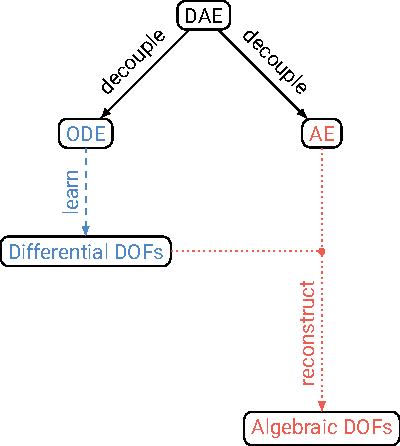
\includegraphics[width=.7\textwidth]{ial}
    \end{center}
    \caption{Schematic workflow of index-aware learning.}
    \label{fig:ial}
\end{figure}

In terms of the example circuits from \autoref{subsec:dcmna} the workflow amounts to the following: for the first example we only consider $\varphi_3$ and $i_\mr{L}$ as variables that need to be learned and for the second example solely $\varphi_3$ is left. All remaining degrees of freedom may be recovered using \eqref{eq:do1} or \eqref{eq:do2} respectively. Thus the learning effort is already reduced quite significantly in these two examples; from five to two variables in the first and from four down to one variable in the second example. Another key benefit comes from the fact that the reconstructed algebraic variables exactly fulfill the inherent constraints of the DAE. This means that even though the learned solution variables (think of $\varphi_3$ for example) are only approximations, the reconstructions (e.g. $\varphi_1$ or $\varphi_2$) will still be consistent. This may be of great importance for systems where the physical interpretability of the solution depends on it satisfying the constraints.

There is yet another, maybe less expected, benefit that might occur. Looking at the decoupled system from \eqref{eq:do2} we find that the resistance parameter $R$ and the inductance parameter $L$ only appear in the algebraic equation. In terms of our original goal of speeding up design optimization or uncertainty quantification, where a lot of solutions for varying parameter values are required, this means the following: instead of needing to solve the full system for a given combination of $R$ and $L$, we can instead merely solve the algebraic equation to obtain the full solution. While the algebraic equation might be more complicated than the simple linear relations of \eqref{eq:do1} and \eqref{eq:do2} in general, solving it is almost certainly much faster than having to integrate the entire system in time. This becomes an even bigger advantage when knowledge about the solution is only required for specific points in time, since the algebraic equation may be solved pointwise.

Lastly, we emphasize that the approach is independent of the particular machine learning technique that is used for predicting the differential DOFs. Thus methods developed especially for ODEs may be employed and exchanged depending on the problem at hand.

\section{Numerical examples}
\label{sec:ne}
Before we present numerical results regarding the two example circuits introduced in \autoref{subsec:dcmna}, we want to provide some background on our machine learning method of choice, Gaussian processes (GPs), and the particular learning strategy we employ.

\paragraph{Gaussian processes}
The following brief introduction is based on the textbook of Rasmussen and Williams\cite{rasmussen2006} and we refer to the book itself for more details. We consider the problem of approximating one component $x(t)$ of the DAE solution $\mb{x}(t)$, compare \eqref{eq:dae}, based on observations
\begin{align*}
    O = \big\{ (t_i, x_i): 1 \leq i \leq N \big\}.
\end{align*}
We will focus on the one-dimensional case for clarity of exposition, however we remark that the ideas extend to the case where the solution component $x(t, \mb{p})$ also depends on the parameters and thus more than one variable, compare also the textbook\cite{rasmussen2006}. A GP suitable for this problem is defined by a (prior) mean function $m: \mathbb{R} \to \mathbb{R}$ and covariance function $k: \mathbb{R} \times \mathbb{R} \to \mathbb{R}$. The learning problem is then tackled using Bayesian inference, such that one aims to obtain the posterior distribution $\hat{x}(t)$, given the observations $O$ and a point $t$, where $x$ is to be predicted. A particular feature of GPs is that this posterior process, under suitable assumptions, turns out to be another GP with posterior mean and covariance\cite{basak2021}
\begin{subequations}
    \label{eq:gp}
    \begin{align}
        \hat{m}(t) &= m(t) + \mb{w}(t)^\T (\mb{x} - \mb{m}) \label{eq:gpm}\\
        \hat{k}(t) &= k(t, t) - \mb{w}(t)^\T \mb{k}(t) \label{eq:gpv},
    \end{align}
\end{subequations}
where $\mb{m} \coloneqq [m(t_1), \dotsc, m(t_N)]^\T$ denotes the prior mean function evaluated at the observations, $\mb{k}(t) \coloneqq [k(t, t_1), \dotsc, k(t, t_N)]^\T$ similarly denotes the pairwise evaluation of the covariance function using the prediction point $t$ and the observations, and $\mb{x} \coloneqq [x_1, \dotsc, x_N]^\T$ are the observed function values. The weights $\mb{w}(t)$ are given by the solution of
\begin{align*}
    \big( \mb{K} + \sigma^2 \mb{I} \big) \mb{w}(t) = \mb{k}(t),
\end{align*}
where $[\mb{K}]_{i,j} \coloneqq k(t_i, t_j)$ and $\sigma^2$ models i.i.d.~additive Gaussian noise on the observations. For a discussion on modeling choices where the assumptions leading to \eqref{eq:gp} are not fulfilled, see the review article by Swiler et al.\cite{swiler2020}.

The key model component influencing the learning process is the covariance (or kernel) function $k$, since it determines the approximation properties of the GP. It encodes prior knowledge about the function $x(t)$ that is to be learned, such as differentiability or characteristic length scales. We opt for a radial basis function kernel, given by
\begin{align*}
    k(t_i, t_j, \sigma_k, \ell) = \sigma_k^2 \exp \biggl(- \Big( \frac{t_i - t_j}{\ell} \Big)^2 \biggr),
\end{align*}
where $\sigma_k$ and the length scale $\ell$ are hyperparameters, which allow for better approximation capabilities of the GP. The kernel is selected to match the differentiability of the solution.

In practice, the mean function $m$ is often taken to be zero as the data is assumed standardized and the hyperparameters are then determined by minimizing the negative log likelihood\cite{basak2021}
\begin{align*}
    -\log \bigl( p(\mb{x} | \sigma, \sigma_k, \ell) \bigr) = \frac{1}{2} \big( \mb{x}^\T \mb{K}(\sigma, \sigma_k, \ell)^{-1} \mb{x} + \log \bigl( \det \mb{K}(\sigma, \sigma_k, \ell) \bigr) + N \log(2\pi) \big),
\end{align*}
where $[\mb{K}(\sigma, \sigma_k, \ell)]_{i,j} \coloneqq k(t_i, t_j, \sigma_k, \ell) + \sigma^2$.

\paragraph{Learning strategy}
The learning strategy aims to exploit one of the key features of GPs: that they provide both a mean prediction $\hat{m}$ and an associated variance estimate $\hat{k}$, as detailed in \eqref{eq:gp}. We use these properties in conjunction with a greedy sample selection strategy, that starts out with a small number of training data points and adds additional samples based on the variance estimate of the GP. This idea is not new, see again the textbook of Rasmussen and Williams\cite{rasmussen2006} for more references and details, however we still want to outline our particular approach to make the results better interpretable and reproducible.

Our implementation proceeds as follows:
\begin{enumerate}
    \item We select a grid of time points $T = \{ t_i: 1 \leq i \leq N_T \}$ and parameter values $P = \{ \mb{p}_i: 1 \leq i \leq N_P \}$, where each $\mb{p}_i$ represents a specific combination of parameter values, for which we want to model the solution of the DAE using a GP.
    \item We select a subset $D \subset T \times P$ and use the corresponding solutions for the initial training of a GP.
    \item As a termination criterion, we compute the posterior mean $\hat{m}(t, \mb{p})$ using \eqref{eq:gpm} in all grid points $(t, \mb{p}) \in T \times P$ and check whether the relative prediction error
    \begin{align*}
        e \coloneqq \frac{\| \mbh{m} - \mb{x} \|_2}{ \| \mb{x} \|_2},
    \end{align*}
    is below a desired tolerance, and if not, continue with 4. Here, $\mbh{m} \coloneqq [\hat{m}(t_1, \mb{p}_1), \dotsc, \hat{m}(t_{N_T}, \mb{p}_{N_P})]$ collects the mean predictions for all $(t, \mb{p}) \in T \times P$ and $\mb{x}$ contains the corresponding simulated solution values.
    \item We compute the variance prediction $\hat{k}(t, \mb{p})$ using \eqref{eq:gpv} for all $(t, \mb{p}) \in (T \times P) \setminus D$ and add the point of maximum variance to the training data set $D$.
    \item Finally, we retrain the model and continue with 3.
\end{enumerate}

We note that several improvements may be made to this strategy, such as properly maximizing the variance estimate in 4, instead of sampling on a discrete grid. The implementation is based on the STK toolbox\cite{stk}.

\paragraph{First example circuit}
We again consider the example of \autoref{fig:do1}, where we choose $R = \SI{500}{\ohm}$, $v_\mr{s}(t) = \sin(600 \pi t)\, \si{\volt}$ and the diode is modeled by $g_\mr{D}(\varphi_3) = 10^{-14} \big( e^{(\varphi_3 / \SI{26}{\mV})} - 1 \big)\, \si{\siemens}$. The remaining parameter values are chosen according to the greedy sample selection strategy with $\SI{1}{\milli\henry} \leq L \leq \SI{3}{\milli\henry}$ and $\SI{100}{\nano\farad} \leq C \leq \SI{300}{\nano\farad}$, i.e.~$\mb{p} = [L\ C]$ in the context of \autoref{sec:int}. The starting points for the strategy are given by all combinations of the boundary values for $L$ and $C$ together with $t = \SI{0}{\ms}$ and $t = \SI{10}{\ms}$ once for each combination. Recalling \eqref{eq:do1}, we see that $\varphi_3$ and $i_\mr{L}$ have to be learned as the differential DOFs. In addition to these two, we also consider the algebraic variable $\varphi_2$ and we will compare the accuracy of learning $\varphi_2$ directly to recovering it from the two differential variables. \autoref{fig:do1_solution} shows the solution for $L = \SI{1.7}{\milli\henry}$ and $C = \SI{220}{\nano\farad}$, a combination which is not part of the training data.
\begin{figure}[t]
    \begin{center}
        \includegraphics[width=.4\textwidth]{do1_solution_phi} \hspace{1.5cm} 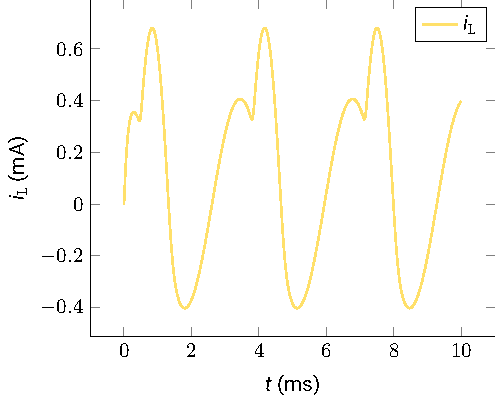
\includegraphics[width=.4\textwidth]{do1_solution_i_L}
    \end{center}
    \caption{Solution of the first example circuit for $L = \SI{1.7}{\milli\henry}$ and $C = \SI{220}{\nano\farad}$.}
    \label{fig:do1_solution}
\end{figure}

\begin{figure}[b]
    \begin{center}
        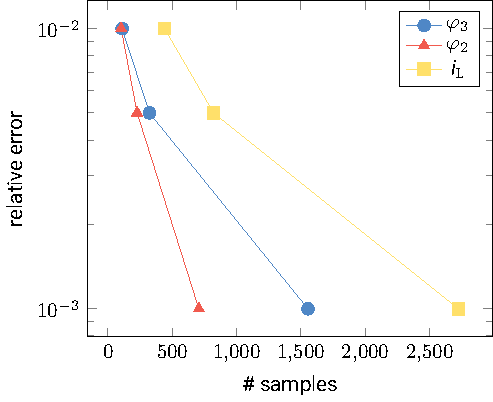
\includegraphics[width=.4\textwidth]{do1_convergence}
    \end{center}
    \caption{Convergence of the relative prediction error $e$, for the variables shown in \autoref{fig:do1_solution}. The final accuracies correspond to approximately 180 different combinations of $L$ and $C$ for $\varphi_3$, 39 combinations for $\varphi_2$ and 37 for $i_\mr{L}$.}
    \label{fig:do1_convergence}
\end{figure}
In \autoref{fig:do1_convergence}, we see the convergence of the relative prediction errors with respect to the number of samples used by the greedy selection strategy. We observe that, depending on the qualitative complexity of the dynamics, the solution variables take different numbers of samples to reach the same prediction accuracy. It should be noted however, that the total number of samples $N_D$ also includes the number of time points that are sampled, and not only the number of distinct parameter combinations (simulations). The latter are listed in the caption of \autoref{fig:do1_convergence} and turn out to be considerably smaller. One may also note that we only execute the learning strategy up to a relatively large tolerance of $10^{-3}$. This is due to the fact that both the optimization of the hyperparameters, as well as the computation of the posterior mean and variance, scale badly for conventional GPs, leading to large computation times. Remedies for this exist, see e.g.~the book by Rasmussen and Williams\cite{rasmussen2006}, however this issue lies outside the scope of this article as our approach may be combined with any machine learning method of choice.
\begin{figure}[t]
    \begin{center}
        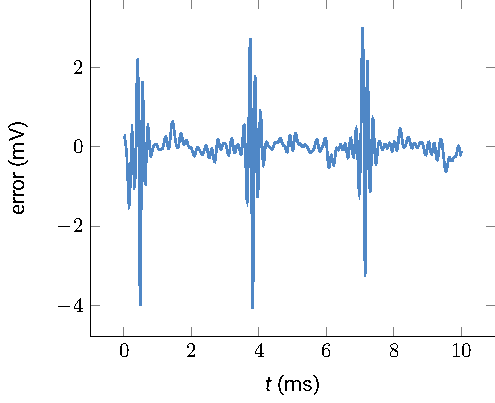
\includegraphics[width=.4\textwidth]{do1_error_phi_3} \hspace{1.5cm} 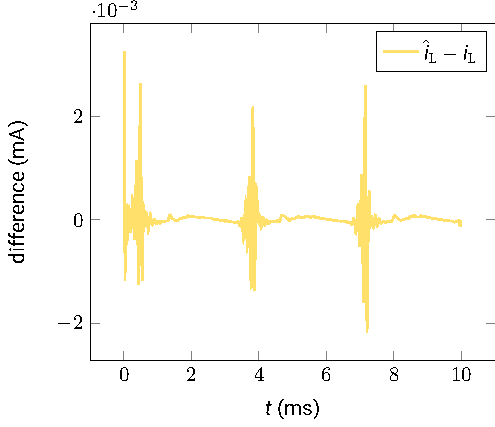
\includegraphics[width=.4\textwidth]{do1_error_i_L}
    \end{center}
    \caption{Differences between the mean predictions ($\hat{\varphi}_3$ and $\hat{i}_\mr{L}$) and the corresponding simulations for the differential variables when considering $L = \SI{1.7}{\milli\henry}$ and $C = \SI{220}{\nano\farad}$. The predictions correspond to the smallest relative errors from \autoref{fig:do1_convergence}.}
    \label{fig:do1_error_d}
\end{figure}

\begin{figure}[b]
    \begin{center}
        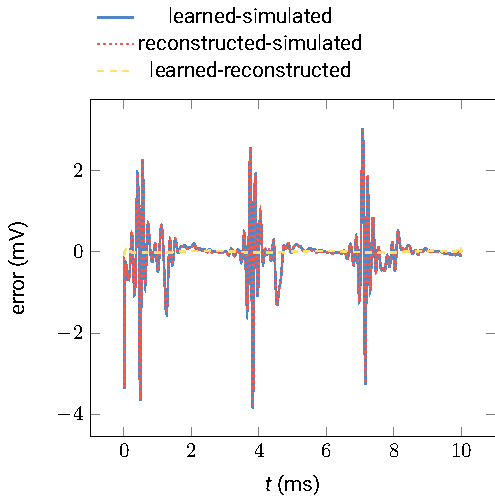
\includegraphics[width=.4\textwidth]{do1_error_phi_2} \hspace{1.5cm} \includegraphics[width=.4\textwidth]{do1_consistency}
    \end{center}
    \caption{Differences between the mean prediction $\hat{\varphi}_2$, reconstruction $\bar{\varphi}_2$ and the corresponding simulation of the algebraic variable $\varphi_2$ (left) and the respective consistency errors (right). The predictions correspond to $L = \SI{1.7}{\milli\henry}$, $C = \SI{220}{\nano\farad}$ and the smallest relative error from \autoref{fig:do1_convergence}.}
    \label{fig:do1_error_a_consistency}
\end{figure}
The differences between the mean predictions and simulations for the differential DOFs, when using the predictions belonging to the smallest relative errors from \autoref{fig:do1_convergence}, are shown in \autoref{fig:do1_error_d}. The results again correspond to $L = \SI{1.7}{\milli\henry}$ and $C = \SI{220}{\nano\farad}$, and we observe that the differences are in line with the relative prediction errors of \autoref{fig:do1_convergence}. The differences between the mean prediction $\hat{\varphi}_2$, reconstruction $\bar{\varphi}_2$ and the simulation of the algebraic variable $\varphi_2$ are highlighted on the left of \autoref{fig:do1_error_a_consistency}. The results again correspond to the same parameter values $L = \SI{1.7}{\milli\henry}$ and $C = \SI{220}{\nano\farad}$. We observe that there is not much difference between the mean prediction and reconstruction, however the reconstruction does appear to have a slight advantage in terms of accuracy. Here, one should note that although the reconstruction is exact up to the accuracy of solving the algebraic equation \eqref{eq:do1}, it still contains the error from learning the differential variables, hence the overall difference between $\bar{\varphi}_2$ and $\varphi_2$. To better quantify the difference between the learned and reconstructed solutions, we therefore introduce consistency errors $\hat{e}(t)$ and $\bar{e}(t)$ based on \eqref{eq:do1}
\begin{align*}
    \hat{e}(t) \coloneqq \begin{Vmatrix}
        \hat{\varphi}_1 - v_\mr{s}\\
        \hat{\varphi}_2 + R \hat{i}_\mr{L} - v_\mr{s}\\
        \hat{i}_\mr{V} + i_\mr{L}
    \end{Vmatrix}_2, \quad \bar{e}(t) \coloneqq \begin{Vmatrix}
        \bar{\varphi}_1 - v_\mr{s}\\
        \bar{\varphi}_2 + R \hat{i}_\mr{L} - v_\mr{s}\\
        \bar{i}_\mr{V} + i_\mr{L}
    \end{Vmatrix}_2,
\end{align*}
where $\hat{\cdot}$ indicates learned quantities and $\bar{\cdot}$ refers to reconstructed quantities. For a consistent solution obeying all algebraic constraints, both errors are identically zero. The right of \autoref{fig:do1_error_a_consistency} shows these consistency errors when using the same predictions and reconstructions as on the left. We observe a very clear improvement of the reconstructions (consistency error on the order of machine precision) over the directly learned predictions (consistency error as large as $10^{-3}$). While the central benefit is of course this adherence to the constraints, only needing to learn two of the five solution variables also represents a significant reduction of the learning effort in this case.

\paragraph{Second example circuit}
For the second example from \autoref{fig:do2}, we select $i_\mr{s}(t) = 10^{-4} \sin(400 \pi t)\, \si{\volt}$, while all other parameters and the learning strategy remain the same. Recalling \eqref{eq:do2}, we find that $\varphi_3$ is the only differential variable that needs to be learned to reconstruct the remaining algebraic DOFs. We again focus on $\varphi_2$ as an algebraic variable to obtain a comparative example.
\begin{figure}[b]
    \begin{center}
        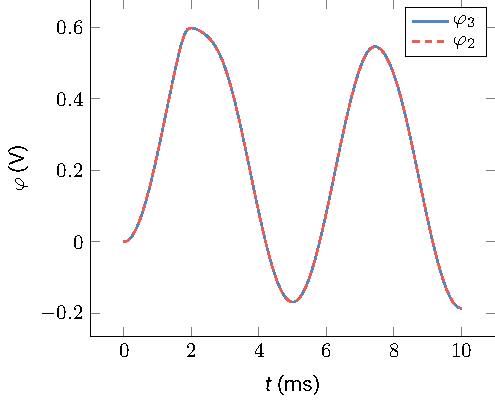
\includegraphics[width=.4\textwidth]{do2_solution_phi} \hspace{1.5cm} 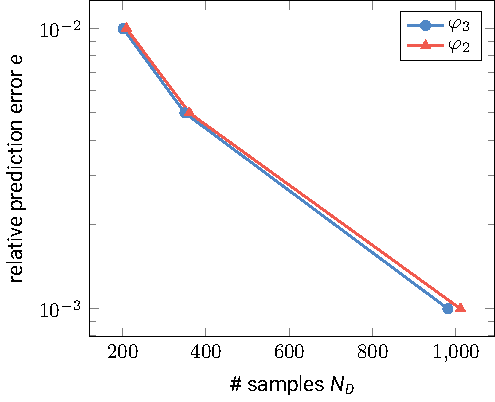
\includegraphics[width=.4\textwidth]{do2_convergence}
    \end{center}
    \caption{Solution of the second example circuit for $L = \SI{1.7}{\milli\henry}$ and $C = \SI{220}{\nano\farad}$ (left) and convergence of the relative prediction error for the same variables (right). The final accuracies correspond to 31 distinct combinations of $L$ and $C$ for $\varphi_3$ and 49 for $\varphi_2$.}
    \label{fig:do2_solution_convergence}
\end{figure}

Considering similar numerical studies as for the first example, the left panel of \autoref{fig:do2_solution_convergence} shows the solutions of $\varphi_3$ and $\varphi_2$ for $L = \SI{1.7}{\milli\henry}$ and $C = \SI{220}{\nano\farad}$, which are again not part of the training data. The right plot shows the convergence of the relative prediction errors with respect to the total number of samples $N_D$. We again note that the number of distinct parameter combinations is significantly smaller, as listed in the caption. We also see that the relative errors behave similarly for both variables in this case, which is to be expected given the similar outlook of their dynamics in the left plot.
\begin{figure}[t]
    \begin{center}
        \includegraphics[width=.4\textwidth]{do2_error_phi_3} \hspace{1.5cm} 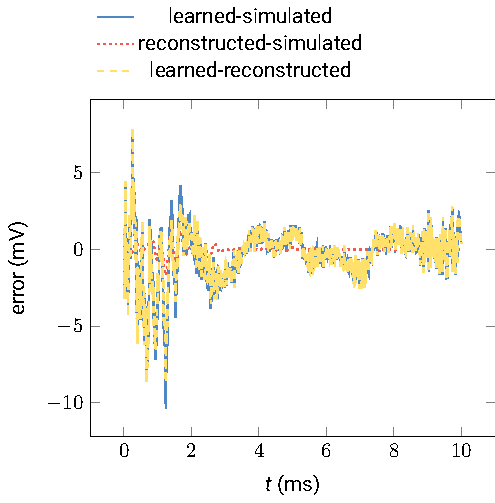
\includegraphics[width=.4\textwidth]{do2_error_phi_2}
    \end{center}
    \caption{Differences between the mean prediction and simulation for $\varphi_3$ (left) and between the mean prediction, reconstruction and simulation for $\varphi_2$ (right). The predictions are again made for $L = \SI{1.7}{\milli\henry}$ and $C = \SI{220}{\nano\farad}$ and correspond to the smallest relative errors from \autoref{fig:do2_solution_convergence}.}
    \label{fig:do2_error}
\end{figure}

\begin{figure}[b]
    \begin{center}
        \includegraphics[width=.4\textwidth]{do2_consistency}
    \end{center}
    \caption{Consistency errors $\hat{e}(t)$ and $\bar{e}(t)$ corresponding to the results from \autoref{fig:do2_error}. The additional term $\check{e}(t)$ refers to the consistency error of the alternative approach, when using the predictions and Euler corrections outlined in \autoref{fig:do2_euler}.}
    \label{fig:do2_consistency}
\end{figure}
At this point we also return to the discussion from \autoref{sec:ial} about parameters only appearing in the algebraic equation. During the learning process, the greedy strategy requested 21 unique values for $C$, all of which required full simulations according to \eqref{eq:do2}. The 7 unique values for $L$, that were requested for learning $\varphi_2$, did not require full simulations however, but rather could be reconstructed from \eqref{eq:do2}. We again emphasize that time is also included as a parameter within the sample selection strategy, such that the reconstruction not only constitutes a reduction from solving a nonlinear DAE in four variables to merely evaluating a scalar equation, but that this scalar equation furthermore only needs to be evaluated at the particular points in time that are requested by the strategy, rather than at all time points of the solution.

The difference between the mean prediction and simulation of $\varphi_3$, for $L = \SI{1.7}{\milli\henry}$ and $C = \SI{220}{\nano\farad}$, is shown on the left of \autoref{fig:do2_error}, while the right shows the differences between the mean prediction, reconstruction and simulation of $\varphi_2$. The predictions again correspond to the smallest relative errors from \autoref{fig:do2_solution_convergence} and the differences are of the same order. In this case, the reconstruction performs similar or even slightly worse compared to the mean prediction when only looking at the difference. However it still constitutes a reduction in learning effort, from four solution variables down to only one, and most importantly it adheres to the algebraic constraints of the DAE. To further illustrate this point, we again take a look at the consistency errors, now redefined based on \eqref{eq:do2}
\begin{align*}
    \hat{e}(t) \coloneqq \begin{Vmatrix}
        \hat{\varphi}_1 - \hat{\varphi}_2 + R i_\mr{s}\\
        \hat{\varphi}_2 - \hat{\varphi}_3 + L \ddt i_\mr{s}\\
        \hat{i}_\mr{L} - i_\mr{s}
    \end{Vmatrix}_2, \quad \bar{e}(t) \coloneqq \begin{Vmatrix}
        \bar{\varphi}_1 - \bar{\varphi}_2 + R i_\mr{s}\\
        \bar{\varphi}_2 - \hat{\varphi}_3 + L \ddt i_\mr{s}\\
        \bar{i}_\mr{L} - i_\mr{s}
    \end{Vmatrix}_2.
\end{align*}
In our example, the algebraic equation from \eqref{eq:do2} gives an explicit description of the algebraic variables once more, such that the reconstruction is accurate up to machine precision, compare $\bar{e}(t)$ in \autoref{fig:do2_consistency}. When learning all solution variables individually however, we observe a much larger maximum value of around $10^{-3}$ for the consistency error $\hat{e}(t)$ across all the predicted points in time. In general, the algebraic equation may be nonlinear such that the reconstruction still leads to a consistency error $\bar{e}(t)$ greater than machine precision, depending on the accuracy of the nonlinear system solver.

\subsection{Alternative approach}
\label{subsec:aa}
In a last step, we want to provide an alternative approach to reducing the consistency error, while avoiding an extra implementation to handle the algebraic constraints. The idea is based on the insight that two successive implicit Euler steps suffice to bring the algebraic variables into a consistent state with the differential ones, when starting with inconsistent initial values\cite{garcia2022}. In our context, one can then simply learn all solution variables independently, and when making a prediction, select a time point slightly before the intended prediction point, such that two small implicit Euler steps may be performed as a correction to obtain a consistent solution.
\begin{figure}[t]
    \begin{center}
        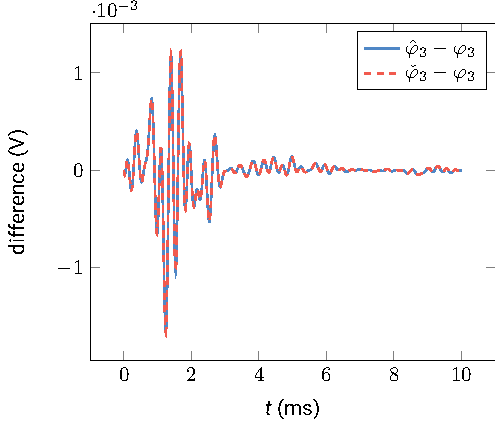
\includegraphics[width=.4\textwidth]{do2_euler_phi_3} \hspace{1.5cm} \includegraphics[width=.4\textwidth]{do2_euler_phi_2}
    \end{center}
    \caption{Differences between the mean predictions, Euler corrections and simulations for $\varphi_3$ (left) and $\varphi_2$ (right). The predictions are made for $L = \SI{1.7}{\milli\henry}$ and $C = \SI{220}{\nano\farad}$ and correspond to the smallest relative errors from \autoref{fig:do2_solution_convergence}.}
    \label{fig:do2_euler}
\end{figure}

This alternative approach has the advantage that it can be directly applied using simulations from any SPICE-like software, and using any machine learning method for the predictions, without worrying about the reconstruction of the algebraic variables. However it may not achieve the same level of accuracy as the approach outlined in \autoref{sec:ial} in practice, depending on the Euler step size and the accuracy of the nonlinear system solver\cite{garcia2022}. Furthermore, it requires predictions for all solution variables, which represents unnecessary computational cost, and there is no chance for parameters to shift completely to the algebraic equations, compare \autoref{sec:ial}.

\autoref{fig:do2_euler} shows the differences between the mean predictions ($\hat{\varphi}_3$, $\hat{\varphi}_2$), Euler corrections ($\check{\varphi}_3$, $\check{\varphi}_2$) and the simulations for the second example, using the same parameters as in \autoref{fig:do2_error}. We see that the two Euler steps have almost no effect on the differential variable $\varphi_3$, as expected. For the algebraic variable $\varphi_2$ however, the mean predictions $\hat{\varphi}_2$ and the corrected predictions after two Euler steps $\check{\varphi}_2$, differ significantly, with the latter resembling the reconstruction from \autoref{fig:do2_error}. Also defining a consistency error $\check{e}(t)$ based on \eqref{eq:do2} in this case
\begin{align*}
    \check{e}(t) \coloneqq \begin{Vmatrix}
        \check{\varphi}_1 - \check{\varphi}_2 + R i_\mr{s}\\
        \check{\varphi}_2 - \check{\varphi}_3 + L \ddt i_\mr{s}\\
        \check{i}_\mr{L} - i_\mr{s}
    \end{Vmatrix}_2
\end{align*}
and comparing it to the other approaches, see \autoref{fig:do2_consistency}, shows that this alternative approach represents a compromise in terms of accuracy in the algebraic constraints. The maximum value of the consistency error $\check{e}(t)$ of the corrected predictions comes out around $10^{-7}$, about four orders of magnitude smaller compared to before the correction. While it is theoretically possible to also force the error down to machine precision in this case, other factors become prohibitive as mentioned earlier.

\section{Conclusions and future research}
\label{sec:cfr}
This article introduced a new method for learning the time and parameter dependent behavior of electrical circuits. The method assumes the circuit to be modeled using MNA and then exploits the structure of MNA to improve the learning process by splitting it into a learning and a reconstruction stage, compare \autoref{fig:ial}. It achieves this by decoupling the underlying DAE into an ODE and a purely algebraic equation. Benefits of the method include a reduction in the number of variables that are to be learned during the learning stage and the exact adherence of the learned solution to the inherent constraints of the circuit model after the reconstruction stage. Two numerical examples illustrated both benefits. The examples also showed that the exact recovery of the constraints might improve the accuracy of the learned solutions. Furthermore, additional computational savings may be possible as some of the parameters of interest only appear in the reconstruction stage, which entirely avoids the need for training data with varying values of these parameters. We emphasize that the approach is independent of the machine learning method used during the learning stage, such that the learning method may be chosen according to the problem at hand. Lastly, we showcased an alternative approach that avoids the need for the decoupling and the associated implementation, while still improving the adherence of the learned solution to the algebraic constraints of the DAE.

Multiple extensions are possible within this index-aware learning framework. A natural first step could be to make use of the topological decomposition that was hinted at in \autoref{sec:dc}. This would pave the way for the inclusion of controlled sources within the workflow, and thus the industrial use of the approach, with the idea being the extension of the topological decomposition to also allow for controlled sources. Focusing in on the idea of adhering to physically meaningful constraints, one could work on extending the concept to a charge conserving variant of MNA, to potentially guarantee charge conservation even for the learned solutions. Yet another direction may be the application of index-aware learning to DAEs arising elsewhere, e.g.~in modified loop analysis. (The dissection concept applies to a more general class of DAEs, as \autoref{sec:dc} showed.) Finally, separate but related work may focus on improving the learning stage by developing new methods that are especially suited for learning ODEs.

\section{Images}
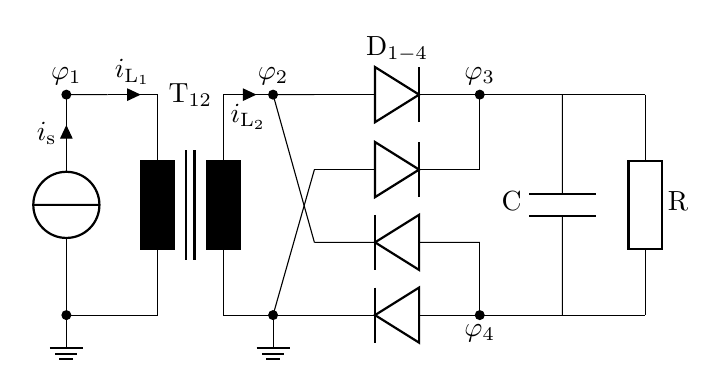
\begin{tikzpicture}
    \def\l{2.1};
    \ctikzset{quadpoles/transformer core/height=2}
    \def\h{2.8};

    \draw (0,0) node[ground] {};
    \draw (0,0) to[I=$i_\mr{s}$, *-*] (0,\h);
    \draw (0.25*\l,0) node[transformer core, anchor=A2] (T) {};
    \draw (T.base) node {$\mr{T}_{12}$};
    \draw (T.B2) node[ground] {};

    \draw (0,\h) to (T.A1);
    \draw (T.A1) to[short, i=$i_{\mr{L}_1}$] ++(right:0.3*\l);
    \draw (0,0) to (T.A2);
    \draw (T.B1) to[short, i<=$i_{\mr{L}_2}$] ++(left:0.3*\l);
    \draw (T.B1) node[circ] {};
    \draw (T.B2) node[circ] {};

    \draw (1.5*\l,\h) to[Do=$\mr{D}_{1-4}$, -*] (2.5*\l,\h);
    \draw (1.5*\l,0.66*\h) to[Do] (2.5*\l,0.66*\h);
    \draw (2.5*\l,0.33*\h) to[Do] (1.5*\l,0.33*\h);
    \draw (2.5*\l,0) to[Do, *-] (1.5*\l,0);

    \draw (T.B1) to (1.5*\l,\h);
    \draw (T.B1) to (1.5*\l,0.33*\h);
    \draw (T.B2) to (1.5*\l,0.66*\h);
    \draw (T.B2) to (1.5*\l,0);
    \draw (2.5*\l,0.66*\h) to (2.5*\l,\h);
    \draw (2.5*\l,0.33*\h) to (2.5*\l,0);

    \draw (3*\l,0) to[C=$\mr{C}$] (3*\l,\h);
    \draw (3.5*\l,\h) to[R=$\mr{R}$] (3.5*\l,0);

    \draw (2.5*\l,\h) to (3.5*\l,\h);
    \draw (2.5*\l,0) to (3.5*\l,0);

    \draw (0,\h) node[above] {$\varphi_1$};
    \draw (T.B1) node[above] {$\varphi_2$};
    \draw (2.5*\l,\h) node[above] {$\varphi_3$};
    \draw (2.5*\l,0) node[below] {$\varphi_4$};
\end{tikzpicture}


% \begin{table}
%     \caption{}
%     \begin{center}
%         \begin{tabular}{}
%             \toprule
%             & &\\
%             \midrule
%             & &\\
%             \bottomrule
%         \end{tabular}
%     \end{center}
%     \begin{tablenotes}
%         \item notes
%     \end{tablenotes}
% \end{table}

% \begin{algorithm}
%     \begin{algorithmic}
%     \end{algorithmic}
% \end{algorithm}

\section*{Acknowledgments}
This work is supported by the Graduate School CE within the Centre for Computational Engineering at Technische Universit{\"a}t Darmstadt and the ECSEL Joint Undertaking (JU) under grant agreement No.~101007319. The JU receives support from the European Union's Horizon 2020 research and innovation programme and the Netherlands, Hungary, France, Poland, Austria, Germany, Italy and Switzerland. Note that this work only reflects the authors' views and that the JU is not responsible for any use that may be made of the information it contains.

% \subsection*{Author contributions}

% \subsection*{Financial disclosure}

\subsection*{Conflict of interest}
The authors declare no potential conflict of interests.

% \section*{Supporting information}

% \appendix
% \section{}

% \nocite{*}
\bibliography{biblio}

\clearpage

\section*{Author biography}
\begin{biography}{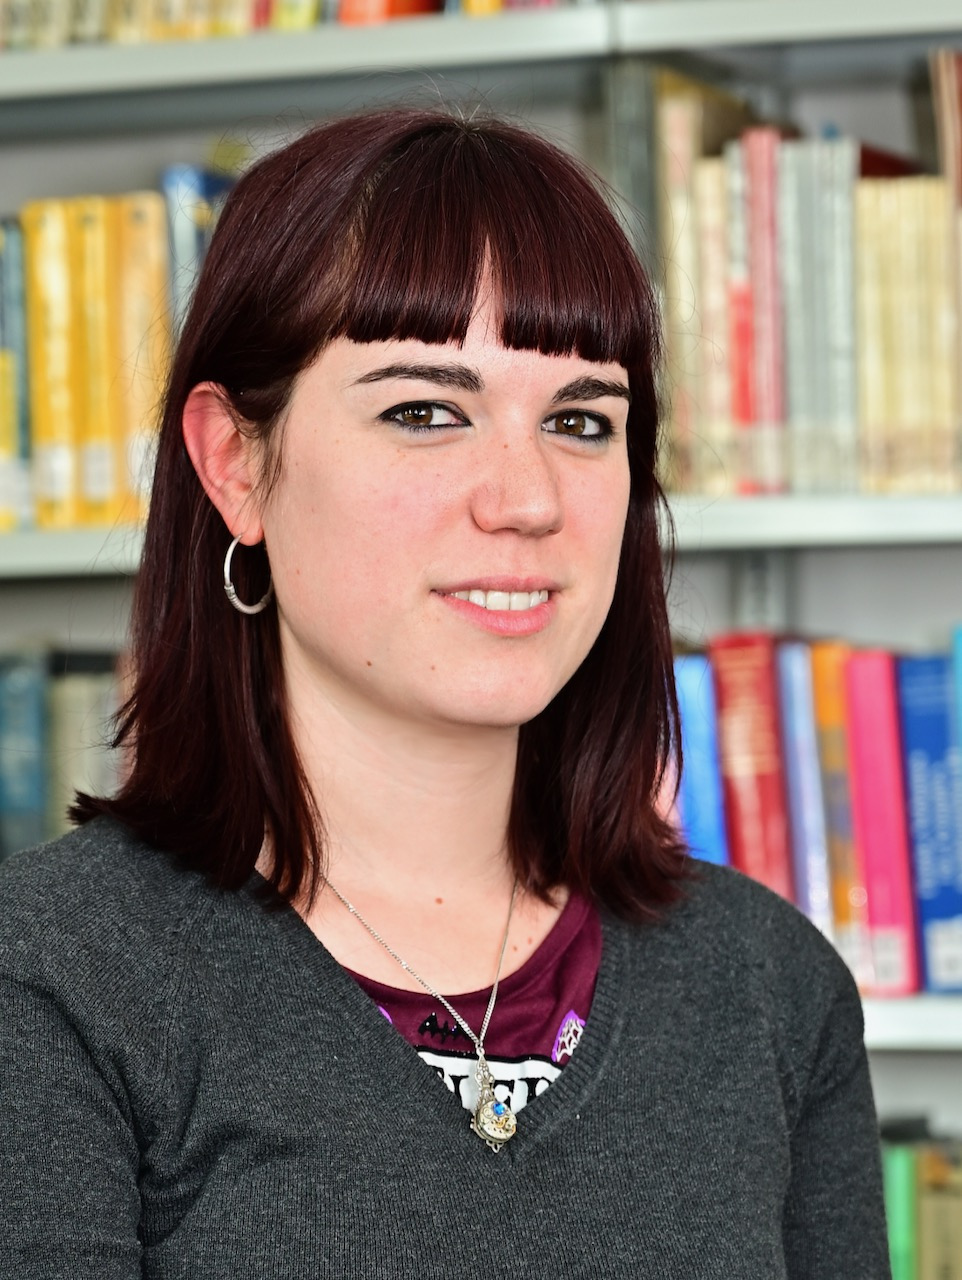
\includegraphics[width=66pt,height=86pt]{cortes}}{\textbf{Idoia Cortes Garcia} received her Bachelor in mathematics and Master in modelling for science and engineering from the Autonomous University of Barcelona. She obtained her Ph.D. in electrical engineering from the Technical University of Darmstadt in 2020. Since 2022 she is an assistant professor at the group of Dynamics and Control from the department of mechanical engineering at Eindhoven University of Technology. Her research interests include coupled multiphysical dynamical systems, differential algebraic equations, efficient time domain (co-)simulation methods and hybrid modelling approaches.}
\end{biography}
\vspace{0.5cm}
\begin{biography}{\includegraphics[width=66pt,height=86pt]{forster}}{\textbf{Peter Förster} received his B.Sc. and M.Sc. degrees in electrical engineering from Technical University of Darmstadt. Currently, he is a doctoral researcher at the centre for analysis, scientific computing and applications at Eindhoven University of Technology and in the computational electromagnetics group at Technical University of Darmstadt. His research interests include circuit simulation, differential-algebraic equations, machine learning and digital twins.}
\end{biography}
\vspace{0.5cm}
\begin{biography}{
\includegraphics[width=66pt,height=86pt]{jansen}}{\textbf{Lennart Jansen} received his M.Sc. degree in mathematics from Universität zu Köln and his Ph.D. degree in mathematics from Universität zu Berlin. Afterwards, he held a post-doc position at Heinrich-Heine-Universität in Düsseldorf before starting work in the industry. One of the main research topics he worked on in the industry was AI-based recommendations for design improvement in the automobile industry. He switched to the photovoltaic industry in 2021 and currently works there on optimal control for combined electric-water-gas networks.}
\end{biography}
\vspace{0.5cm}
\begin{biography}{\includegraphics[width=66pt,height=86pt]{schilders}}{\textbf{Wil Schilders} received the M.Sc. degree in mathematics from Radboud University Nijmegen, Nijmegen, The Netherlands, in 1978, and the Ph.D. degree from the Trinity College Dublin, Dublin, Ireland, in 1980. He has been working in the electronics industry with Philips Research Laboratories, Eindhoven, The Netherlands, since 1980, and NXP, since 2006, where he developed algorithms for simulating semiconductor devices, electronic circuits, organic light emitting diodes, and electromagnetic problems (TV tubes, interconnects, and magnetic resonance imaging). Since 1999, he has been a Part-Time Professor of numerical mathematics for industry with the Technical University of Eindhoven, Eindhoven. He is currently the Managing Director of the Platform for Mathematics in The Netherlands. He is also the President of the European Consortium for Mathematics in Industry.}
\end{biography}
\vspace{0.5cm}
\begin{biography}{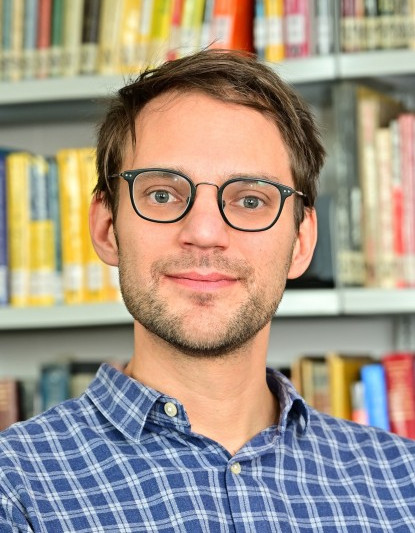
\includegraphics[width=66pt,height=86pt]{schoeps}}{\textbf{Sebastian Schöps} received the M.Sc. degree in business mathematics and the joint Ph.D. degree from Bergische Universität Wuppertal and Katholieke Universiteit Leuven in mathematics and physics. He was appointed as a Professor of Computational Electromagnetics at Technische Universität Darmstadt within the interdisciplinary center of computational engineering, in 2012. His current research interests include coupled multi-physical problems, bridging computer aided design and simulation, parallel algorithms for high performance computing, digital twins, uncertainty quantification, and machine learning.}
\end{biography}

\end{document}
